\problemname{Garbage Collection}

The North Sea is littered with $N$ pieces of garbage, numbered $1 \dots N$.
The $i$'th piece is at position $(x_i, y_i)$ and has a weight of $w_i$.
As part of a cleanup effort, all garbage within a rectangular area will be collected.
This area has a width of $W$ and a height of $H$, but its location has not yet been decided.

Determine the maximum total weight of garbage that will be collected if the cleanup area is positioned optimally.

\section*{Input}
The first line contains the integers $N$, $W$ and $H$.

The $i$'th of the next $N$ lines contains the integers $x_i$, $y_i$ and $w_i$.

\section*{Output}
Print an integer: the maximum total weight of garbage that can be collected.

\section*{Constraints}
\begin{itemize}
  \item $1 \le N \le 10^5$.
  \item $1 \le W, H \le 10^9$.
  \item $0 \le x_i, y_i \le 10^9$ for all $i : 1 \le i \le N$.
  \item $1 \le w_i \le 10^9$ for all $i : 1 \le i \le N$.
\end{itemize}

\section*{Subtasks}
\begin{enumerate}
  \item (10 points) $N \le 400$.
  \item (12 points) $W, H, x_i, y_i \le 2000$ for all $i : 1 \le i \le N$.
  \item (15 points) $N \le 2000$.
  \item (22 points) $H = 10^9$.
  \item (23 points) $W, H, x_i, y_i \le 10^5$ for all $i : 1 \le i \le N$.
  \item (18 points) No additional constraints.
\end{enumerate}

\paragraph{Explanation of Sample}
The optimal area is the one covering the garbage at $(3,1)$, $(2,1)$ and $(1,0)$ with a total weight of $10 + 5 + 5 = 20$.

\begin{center}
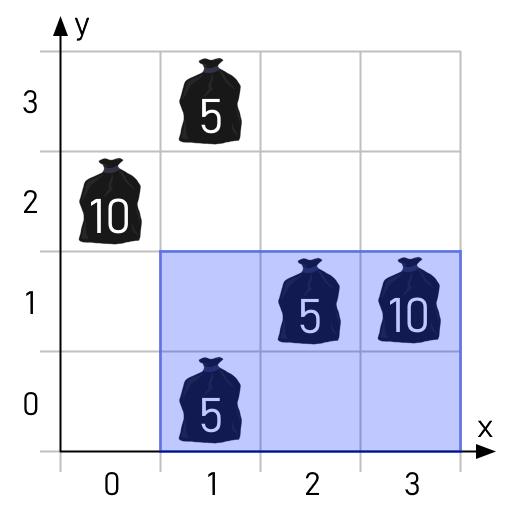
\includegraphics[width=0.6\textwidth]{Figure1.png}
\end{center}
